\chapter{Resultados}

Simulações foram realizadas para testar os dispositivos projetados. Os testes avaliaram o funcionamento geral do circuito de acordo com as especificações do projeto, e também o funcionamento dos componentes APS e TIA.

Para a realização das simulações, é necessário se realizar uma estimativa da fotocorrente gerada dos fotodiodos. Como até o momento da simulação não havia a disponibilidade de uma amostra do fotodiodo, o autor fez uma estimativa conforme o trabalho de \cite{LidianeCampos}, apresentado na \autoref{tab_estcur}.

\begin{table}[!h]
\caption{Estimativa de faixa de fotocorrente gerada}
\label{tab_estcur}
\centering
\begin{tabular}{cc}
\toprule
& Corrente nA \\
\midrule \midrule
Mínimo & 0,1\\
\midrule
Máximo & 30\\
\bottomrule
\end{tabular}
\legend{Fonte: Produzido pelo autor baseado no trabalho \cite{LidianeCampos}}
\end{table}

\section{Máximo sinal DC do APS}
\label{DCAPS}

É avaliado qual é o sinal DC que o bloco APS apresenta sem ter nenhuma fotocorrente gerada, $T_{enable}$ desabilitado e $T_{reset}$ habilitado. Na situação $V_{cn}$ irá apresentar o valor de VDD, o que vai representar o máximo sinal possível em $V_{out}$. A corrente \textit{Iref} considerada foi de $500$ nA, fornecida pelo bloco \textit{current\_mirror\_nmos}. Uma carga de $100$ fF foi utilizada na saída do APS de forma a simular a conexão com  um transistor na saída. O valor obtido foi de $1,15813$ V para $V_{out}$, valor que representa está dentro de VDD menos V\textsubscript{GS} do $T_{buffer}$.

\section{Análise transiente do sinal de saída do APS}

É avaliado qual a resposta do APS com a presença de uma fotocorrente. Para a simulação, foi considerado o modelo apresentado na \autoref{fig_APS_cap}, do qual há uma fonte de corrente em paralelo a um diodo representando a fotogeração. A corrente \textit{Iref} considerada foi de $500$ nA, fornecida pelo bloco \textit{current\_mirror\_nmos}. A tensão de referência de comparação utilizada nas simulações foi de 400 mV.

O Período de Reset nas simulações é definido para ter uma duração de $1$ us. Dois cenários de simulação são descritos nas subseções \ref{sub_sec121} e \ref{sub_sec247} são apresentados, sendo suficientes para comprovação da operação do circuito. O primeiro cenário modela o sinal de fotocorrente gerada com uma onda quadrada de 8 kHz (período de 125 $\mu$s) e valor de amplitude de 5 nA. O segundo cenário modela o sinal de fotocorrente gerada com uma onda quadrada de 4 kHz (período de 250 $\mu$s) e valor de amplitude de 2,5 nA. Esses e outros valores de corrente fotogeradas sugeridos pelo trabalho \cite{LidianeCampos} foram testados na topologia implementada.

\subsection{Período de Integração igual a 121 $\mu$s}
\label{sub_sec121}

Nessa situação, foi considerado uma fotocorrente de 5 nA, que está dentro da faixa proposta pelo autor na \autoref{tab_estcur}. Os resultados obtidos são observados nos gráficos abaixo.

As figuras \ref{graf125}, \ref{graf125z} e \ref{graf1252} apresentam o comportamento esperado entre os Estágios 1 e 2 descritos na \autoref{estagiosAPS}. Assim que RESET é desabilitado (vai para nível lógico '1'), Vout\_analogico passa a decair linearmente, como mostra \autoref{eq_modEletFotIl}. Quando Vout\_analogico atinge o valor de Vref, Vout\_digital vai do nível lógico '0' para '1', como descrito na \autoref{sec_apsdigitalized}.

Note que o RESET habilitado apresenta uma resposta de 'Vout\_analog' com um Overshoot, ou seja, o valor de saída passa por um valor máximo que decai até estabilizar. Isso deve ser levado em conta na medição do circuito real, de forma que o medidor deve limitar o valor máximo de medida a pelo menos o pico no Overshoot para apresentar uma resposta coerente.

\begin{figure}[!h]
 \centering
    \centering
    \caption{Tensão de saída analógica junto aos sinais de RESET e ENABLE para Período de Integração igual a 121 $\mu$s}
    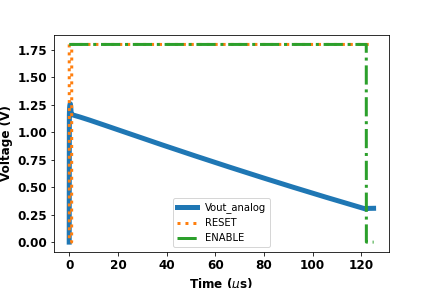
\includegraphics[scale=0.6]{Resultados/Graficos/reseteenable-tb_pixel125.png}
    \legend{Fonte: Produzido pelo autor}
    \legend{Nota: Vout\_analogico representa a tensão de saída analógica do APS}
    \label{graf125}
\end{figure}

\begin{figure}[!h]
 \centering
    \centering
    \caption{Tensão de saída analógica junto aos sinais de RESET e ENABLE para Período de Integração igual a 121 $\mu$s. Ampliado para destacar o sinal de RESET}
    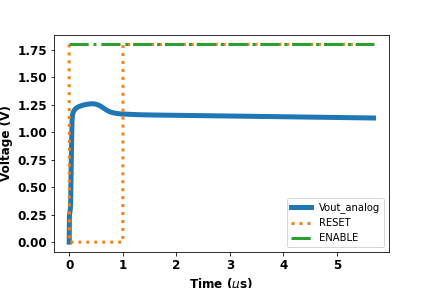
\includegraphics[scale=0.6]{Resultados/Graficos/reseteenable-tb_pixel125_zoom.png}
    \legend{Fonte: Produzido pelo autor}
    \legend{Nota: Vout\_analogico representa a tensão de saída analógica do APS}
    \label{graf125z}
\end{figure}'

\begin{figure}[!h]
 \centering
    \caption{Tensão de saída analógica e tensão de saída digital comparado à tensão de referência do Comparador Período de Integração igual a 121 $\mu$s} 
    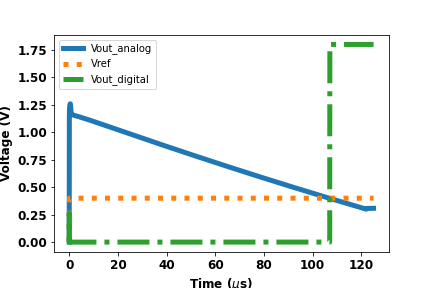
\includegraphics[scale=0.6]{Resultados/Graficos/analogicoedigital-tb_pixel125.png}
    \legend{Fonte: Produzido pelo autor}
    \legend{Nota: Vout\_digital representa a tensão de saída digital do APS\_digitalized}
    \label{graf1252}
\end{figure}

\section{Período de Integração igual a 247 $\mu$s}
\label{sub_sec247}

Nessa situação, foi considerado uma fotocorrente de 2.5 nA, que está dentro da faixa proposta pelo autor na \autoref{tab_estcur}. Os resultados obtidos são observados nos gráficos abaixo.

As figuras \ref{graf247} e \ref{graf2472} apresentam mesmo comportamento daqueles apresentados na \autoref{sub_sec121}, como esperado.

\begin{figure}[!h]
 \centering
    \centering
    \caption{Tensão de saída analógica junto aos sinais de RESET e ENABLE para Período de Integração igual a 247 $\mu$s}
    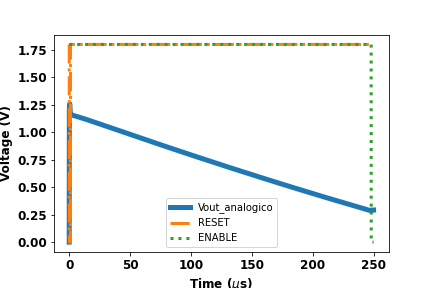
\includegraphics[scale=0.6]{Resultados/Graficos/reseteenable-tb_pixel250.png}
    \legend{Fonte: Produzido pelo autor}
    \legend{Nota: Vout\_analogico representa a tensão de saída analógica do APS}
    \label{graf247}
\end{figure}

\begin{figure}[!h]
 \centering
    \centering
    \caption{Tensão de saída analógica junto aos sinais de RESET e ENABLE para Período de Integração igual a 247 $\mu$s. Ampliado para destacar o sinal de RESET}
    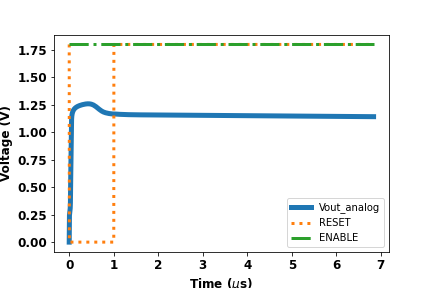
\includegraphics[scale=0.6]{Resultados/Graficos/reseteenable-tb_pixel250_zoom.png}
    \legend{Fonte: Produzido pelo autor}
    \legend{Nota: Vout\_analogico representa a tensão de saída analógica do APS}
    \label{graf247z}
\end{figure}

\begin{figure}[!h]
 \centering
    \caption{Tensão de saída analógica e tensão de saída digital comparado à tensão de referência do Comparador Período de Integração igual a 247 $\mu$s} 
    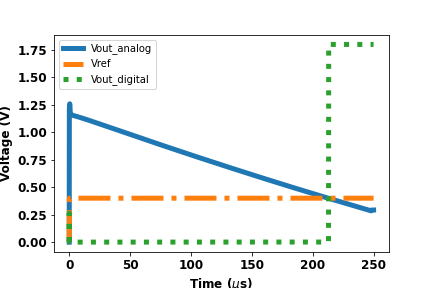
\includegraphics[scale=0.6]{Resultados/Graficos/analogicoedigital-tb_pixel250.png}
    \legend{Fonte: Produzido pelo autor}
    \legend{Nota: Vout\_digital representa a tensão de saída digital do APS\_digitalized}
    \label{graf2472}
\end{figure}

\section{Avaliação de ruído do APS\_digitalized}

Uma simulação para verificar a resposta ao ruído do APS\_digitalized foi realizado, de forma a verificar como variações das respostas dos componentes por efeitos térmicos, ruído flicker e variações dos parâmetros podem impactar a resposta do sistema.

Uma simulação de 1000 iterações foi realizada gerando diferentes variações nos parâmetros dos componentes do sistema e diferentes níveis de ruído. Os perfis de nível de ruído aplicado na saída em cada interação podem ser observado na \autoref{grafruido}. Nas simulações $T_{reset}$ e $T_{enable}$ se mantiveram habilitados, e a intenção foi observar qual foi a variação do máximo valor de tensão que o APS apresenta no Estágio 1.

\begin{figure}[!h]
 \centering
    \caption{Iterações de ruídos na faixa de 1 mV realizadas para simulação} 
    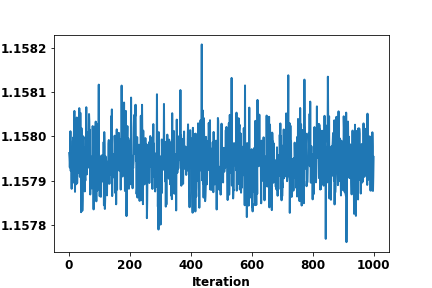
\includegraphics[scale=0.6]{Resultados/Graficos/ruido-Vout_noise.png}
    \legend{Fonte: Produzido pelo autor}
    \label{grafruido}
\end{figure}

O autor do trabalho selecionou aleatoriamente 5 amostras do qual são demonstradas na \autoref{grafruido2}, mas que são suficientes para as conclusões oferecidas.

\begin{figure}[!h]
 \centering
    \caption{Simulações de gráfico de ruído} 
    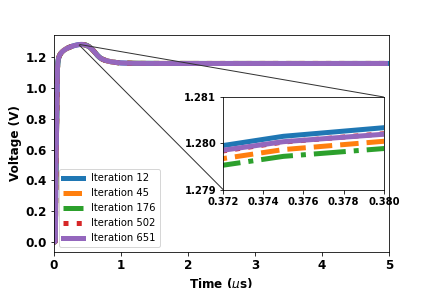
\includegraphics[scale=0.6]{Resultados/Graficos/tb_pixel_TRAN_NOISE.png}
    \legend{Fonte: Produzido pelo autor}
    \label{grafruido2}
\end{figure}

Como pode ser observado pela \autoref{grafruido2}, o ruído não impactou de forma visível a resposta do circuito, aparentando estarem todos visualmente sobre a mesma linha do gráfico. Isso significa, que o impacto de ruídos dos mais diferentes tipos é desprezível para a aplicação, estando na ordem de 1 mV.

\section{Análise transiente do sinal de saída do TIA}

Uma simulação do TIA foi realizada para averiguar se seu comportamento se apresenta adequado. Para as simulações foi utilizado Vref\_amp igual a 800 mV, de forma a polarizar reversamente o fotodiodo e consequentemente aumenta a sua região de depleção, além de sua linearidade; e Vref\_comp igual a 1.3 V utilizado como tensão de referência de comparação no processo de digitalização do comparador. A \autoref{graf_tiasinal} mostra a simulação realizada.

\begin{figure}[!h]
 \centering
    \caption{Tensão de saída analógica do TIA} 
    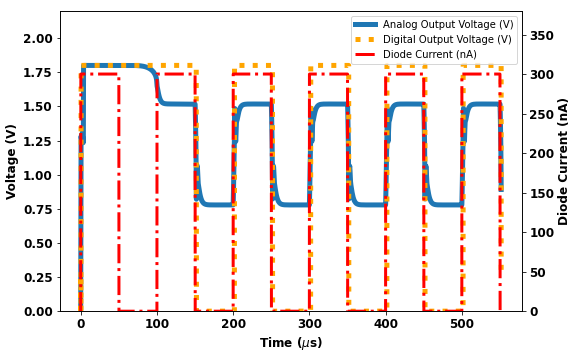
\includegraphics[scale=0.5]{Resultados/Graficos/tb_clock.png}
    \legend{Fonte: Produzido pelo autor}
    \label{graf_tiasinal}
\end{figure}

O comportamento dos gráficos mostra um resultado adequado. Para uma fotocorrente de sinal quadrado, uma tensão quadrada de mesmo formato é gerada para a saída analógica e a digital, após o período inicial de transiente.

\begin{figure}[!h]
 \centering
    \caption{Tensão de saída analógica do TIA. Destaque para o período de subida do sinal de saída analógico.} 
    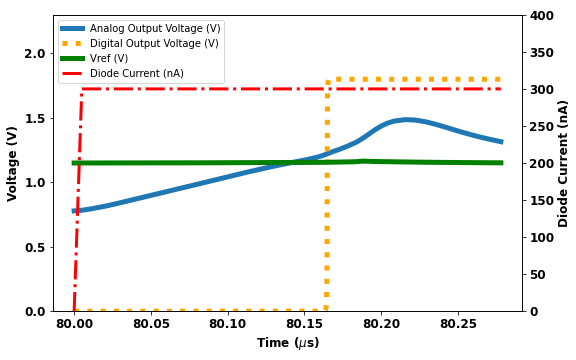
\includegraphics[scale=0.5]{Resultados/Graficos/tb_clock_vref.png}
    \legend{Fonte: Produzido pelo autor}
    \label{graf_tiasinal2}
\end{figure}

\begin{figure}[!h]
 \centering
    \caption{Tensão de saída analógica do TIA. Destaque para o período de descida do sinal de saída analógico.}
    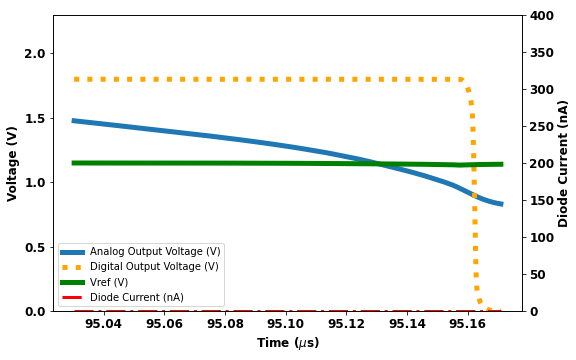
\includegraphics[scale=0.5]{Resultados/Graficos/tb_clock_vref2.png}
    \legend{Fonte: Produzido pelo autor}
    \label{graf_tiasinal3}
\end{figure}

Nota-se das figuras \ref{graf_tiasinal2} e \ref{graf_tiasinal3} que a partir do momento que a tensão analógica cruza o valor da tensão de referência, o valor de tensão digital muda instantes após de forma a apresentar nível lógico '1' quando a tensão analógica estiver subindo, e nível lógico '0' quando estiver caindo.